\documentclass{standalone}
\usepackage{tikz}
\usetikzlibrary{decorations.pathreplacing,decorations.pathmorphing}
\usetikzlibrary{fit,quotes}
\usepackage{yquant, braket}

\begin{document}

%! \usetikzlibrary{decorations.pathreplacing,decorations.pathmorphing}
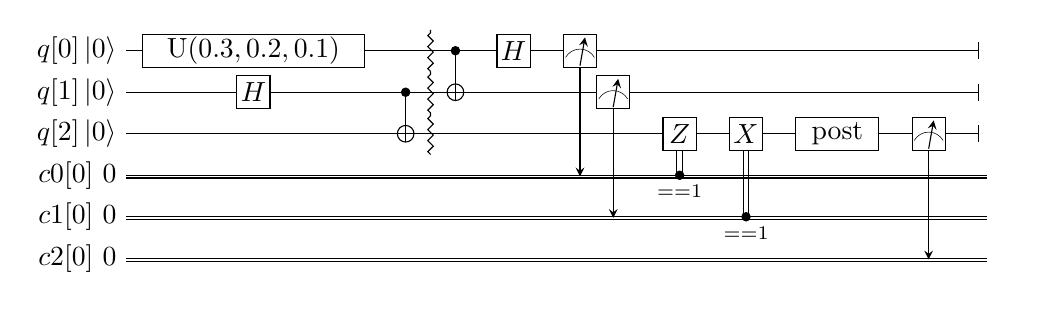
\begin{tikzpicture}[scale=1.000000,x=1pt,y=1pt]
\filldraw[color=white] (0.000000, -7.500000) rectangle (320.000000, 82.500000);
% Drawing wires
% Line 1: q0 W q[0]\ket{0}
\draw[color=black] (0.000000,75.000000) -- (164.000000,75.000000);
%\draw[color=black] (164.000000,74.500000) -- (311.000000,74.500000);
\draw[color=black] (164.000000,75.00000) -- (311.000000,75.00000);
\draw[color=black] (0.000000,75.000000) node[left] {$q[0]\ket{0}$};
% Line 2: q1 W q[1]\ket{0}
\draw[color=black] (0.000000,60.000000) -- (176.000000,60.000000);
%\draw[color=black] (176.000000,59.500000) -- (311.000000,59.500000);
\draw[color=black] (176.000000,60.00000) -- (311.000000,60.00000);
\draw[color=black] (0.000000,60.000000) node[left] {$q[1]\ket{0}$};
% Line 3: q2 W q[2]\ket{0}
\draw[color=black] (0.000000,45.000000) -- (290.000000,45.000000);
%\draw[color=black] (290.000000,44.500000) -- (311.000000,44.500000);
\draw[color=black] (290.000000,45.00000) -- (311.000000,45.00000);
\draw[color=black] (0.000000,45.000000) node[left] {$q[2]\ket{0}$};
% Line 4: c00 W c0[0]\ 0
\draw[color=black] (0.000000,30.000000) -- (311.000000,30.000000);
\draw[color=black] (0.000000,29.000000) -- (311.000000,29.000000);
\draw[color=black] (0.000000,30.000000) node[left] {$c0[0]\ 0$};
% Line 5: c10 W c1[0]\ 0
\draw[color=black] (0.000000,15.000000) -- (311.000000,15.000000);
\draw[color=black] (0.000000,14.000000) -- (311.000000,14.000000);
\draw[color=black] (0.000000,15.000000) node[left] {$c1[0]~0$};
% Line 6: c20 W c2[0]\ 0
\draw[color=black] (0.000000,0.000000) -- (311.000000,0.000000);
\draw[color=black] (0.000000,-1.000000) -- (311.000000,-1.000000);
\draw[color=black] (0.000000,0.000000) node[left] {$c2[0]\ 0$};
% Done with wires; drawing gates
% Line 7: q0 G {U($0.3,0.2,0.1$)} width=80
\begin{scope}
\draw[fill=white] (46.000000, 75.000000) +(-45.000000:56.568542pt and 8.485281pt) -- +(45.000000:56.568542pt and 8.485281pt) -- +(135.000000:56.568542pt and 8.485281pt) -- +(225.000000:56.568542pt and 8.485281pt) -- cycle;
\clip (46.000000, 75.000000) +(-45.000000:56.568542pt and 8.485281pt) -- +(45.000000:56.568542pt and 8.485281pt) -- +(135.000000:56.568542pt and 8.485281pt) -- +(225.000000:56.568542pt and 8.485281pt) -- cycle;
\draw (46.000000, 75.000000) node {{U($0.3,0.2,0.1$)}};
\end{scope}
% Line 8: q1 H
\begin{scope}
\draw[fill=white] (46.000000, 60.000000) +(-45.000000:8.485281pt and 8.485281pt) -- +(45.000000:8.485281pt and 8.485281pt) -- +(135.000000:8.485281pt and 8.485281pt) -- +(225.000000:8.485281pt and 8.485281pt) -- cycle;
\clip (46.000000, 60.000000) +(-45.000000:8.485281pt and 8.485281pt) -- +(45.000000:8.485281pt and 8.485281pt) -- +(135.000000:8.485281pt and 8.485281pt) -- +(225.000000:8.485281pt and 8.485281pt) -- cycle;
\draw (46.000000, 60.000000) node {$H$};
\end{scope}
% Line 9: +q2 q1
\draw (101.000000,60.000000) -- (101.000000,45.000000);
\begin{scope}
\draw[fill=white] (101.000000, 45.000000) circle(3.000000pt);
\clip (101.000000, 45.000000) circle(3.000000pt);
\draw (98.000000, 45.000000) -- (104.000000, 45.000000);
\draw (101.000000, 42.000000) -- (101.000000, 48.000000);
\end{scope}
\filldraw (101.000000, 60.000000) circle(1.500000pt);
% Line 10: q0 BARRIER
\draw[decorate,decoration={zigzag,amplitude=1pt,segment length=4}] (110.000000,67.500000) -- (110.000000,82.500000);
% Line 11: q1 BARRIER
\draw[decorate,decoration={zigzag,amplitude=1pt,segment length=4}] (110.000000,52.500000) -- (110.000000,67.500000);
% Line 12: q2 BARRIER
\draw[decorate,decoration={zigzag,amplitude=1pt,segment length=4}] (110.000000,37.500000) -- (110.000000,52.500000);
% Line 13: +q1 q0
\draw (119.000000,75.000000) -- (119.000000,60.000000);
\begin{scope}
\draw[fill=white] (119.000000, 60.000000) circle(3.000000pt);
\clip (119.000000, 60.000000) circle(3.000000pt);
\draw (116.000000, 60.000000) -- (122.000000, 60.000000);
\draw (119.000000, 57.000000) -- (119.000000, 63.000000);
\end{scope}
\filldraw (119.000000, 75.000000) circle(1.500000pt);
% Line 14: q0 H
\begin{scope}
\draw[fill=white] (140.000000, 75.000000) +(-45.000000:8.485281pt and 8.485281pt) -- +(45.000000:8.485281pt and 8.485281pt) -- +(135.000000:8.485281pt and 8.485281pt) -- +(225.000000:8.485281pt and 8.485281pt) -- cycle;
\clip (140.000000, 75.000000) +(-45.000000:8.485281pt and 8.485281pt) -- +(45.000000:8.485281pt and 8.485281pt) -- +(135.000000:8.485281pt and 8.485281pt) -- +(225.000000:8.485281pt and 8.485281pt) -- cycle;
\draw (140.000000, 75.000000) node {$H$};
\end{scope}
% Line 15: TOUCH
% Line 16: q0:cwire +c00
%\draw (163.500000,75.000000) -- (163.500000,30.000000);
\draw (164.00000,75.000000) -- (164.00000,40.000000);
\filldraw (164.000000, 75.000000) circle(1.500000pt);
\begin{scope}
%\draw[fill=white] (164.000000, 30.000000) circle(3.000000pt);
\clip (164.000000, 30.000000) circle(3.000000pt);
\draw (161.000000, 30.000000) -- (167.000000, 30.000000);
%\draw (164.000000, 27.000000) -- (164.000000, 33.000000);
\end{scope}
\draw[fill=white] (158.000000, 69.000000) rectangle (170.000000, 81.000000);
\draw[very thin] (164.000000, 75.600000) arc (90:150:6.000000pt);
\draw[very thin] (164.000000, 75.600000) arc (90:30:6.000000pt);
\draw[->,>=stealth] (164.000000, 69.600000) -- +(80:10.392305pt);
% Line 17: q1:cwire +c10
%\draw (175.500000,60.000000) -- (175.500000,15.000000);
\draw (176.00000,60.000000) -- (176.00000,25.000000);
\filldraw (176.000000, 60.000000) circle(1.500000pt);
\begin{scope}
%\draw[fill=white] (176.000000, 15.000000) circle(3.000000pt);
\clip (176.000000, 15.000000) circle(3.000000pt);
\draw (173.000000, 15.000000) -- (179.000000, 15.000000);
%\draw (176.000000, 12.000000) -- (176.000000, 18.000000);
\end{scope}
\draw[fill=white] (170.000000, 54.000000) rectangle (182.000000, 66.000000);
\draw[very thin] (176.000000, 60.600000) arc (90:150:6.000000pt);
\draw[very thin] (176.000000, 60.600000) arc (90:30:6.000000pt);
\draw[->,>=stealth] (176.000000, 54.600000) -- +(80:10.392305pt);
% Line 18: q2 Z c00 %% ==1
\draw (224.000000, 15.00000) node[text width=144pt,below,text centered] {\scriptsize ==1};
\draw (199.000000,45.000000) -- (199.000000,30.000000);
\draw (201.000000,45.000000) -- (201.000000,30.000000);
\begin{scope}
\draw[fill=white] (200.000000, 45.000000) +(-45.000000:8.485281pt and 8.485281pt) -- +(45.000000:8.485281pt and 8.485281pt) -- +(135.000000:8.485281pt and 8.485281pt) -- +(225.000000:8.485281pt and 8.485281pt) -- cycle;
\clip (200.000000, 45.000000) +(-45.000000:8.485281pt and 8.485281pt) -- +(45.000000:8.485281pt and 8.485281pt) -- +(135.000000:8.485281pt and 8.485281pt) -- +(225.000000:8.485281pt and 8.485281pt) -- cycle;
\draw (200.000000, 45.000000) node {$Z$};
\end{scope}
\filldraw (200.000000, 30.000000) circle(1.500000pt);
% Line 19: q2 X c10 %% ==1
\draw (200.000000, 30.00000) node[text width=144pt,below,text centered] {\scriptsize ==1};
\draw (223.000000,45.000000) -- (223.000000,15.000000);
\draw (225.000000,45.000000) -- (225.000000,15.000000);
\begin{scope}
\draw[fill=white] (224.000000, 45.000000) +(-45.000000:8.485281pt and 8.485281pt) -- +(45.000000:8.485281pt and 8.485281pt) -- +(135.000000:8.485281pt and 8.485281pt) -- +(225.000000:8.485281pt and 8.485281pt) -- cycle;
\clip (224.000000, 45.000000) +(-45.000000:8.485281pt and 8.485281pt) -- +(45.000000:8.485281pt and 8.485281pt) -- +(135.000000:8.485281pt and 8.485281pt) -- +(225.000000:8.485281pt and 8.485281pt) -- cycle;
\draw (224.000000, 45.000000) node {$X$};
\end{scope}
\filldraw (224.000000, 15.000000) circle(1.500000pt);
% Line 20: q2 G {post} width=30
\begin{scope}
\draw[fill=white] (257.000000, 45.000000) +(-45.000000:21.213203pt and 8.485281pt) -- +(45.000000:21.213203pt and 8.485281pt) -- +(135.000000:21.213203pt and 8.485281pt) -- +(225.000000:21.213203pt and 8.485281pt) -- cycle;
\clip (257.000000, 45.000000) +(-45.000000:21.213203pt and 8.485281pt) -- +(45.000000:21.213203pt and 8.485281pt) -- +(135.000000:21.213203pt and 8.485281pt) -- +(225.000000:21.213203pt and 8.485281pt) -- cycle;
\draw (257.000000, 45.000000) node {{post}};
\end{scope}
% Line 21: q2:cwire +c20
%\draw (289.500000,45.000000) -- (289.500000,0.000000);
\draw (290.00000,45.000000) -- (290.00000,0.000000);
\filldraw (290.000000, 45.000000) circle(1.500000pt);
\begin{scope}
%\draw[fill=white] (290.000000, 0.000000) circle(3.000000pt);
\clip (290.000000, 0.000000) circle(3.000000pt);
\draw (287.000000, 0.000000) -- (293.000000, 0.000000);
%\draw (290.000000, -3.000000) -- (290.000000, 3.000000);
\end{scope}
\draw[fill=white] (284.000000, 39.000000) rectangle (296.000000, 51.000000);
\draw[very thin] (290.000000, 45.600000) arc (90:150:6.000000pt);
\draw[very thin] (290.000000, 45.600000) arc (90:30:6.000000pt);
\draw[->,>=stealth] (290.000000, 39.600000) -- +(80:10.392305pt);
% Line 22: TOUCH
% Line 23: q0 OUT 0
\filldraw[color=white] (308.000000, 72.000000) rectangle (314.000000, 78.000000);
\draw (308.000000, 72.000000) -- (308.000000, 78.000000);
%\draw (311.000000, 75.000000) node {$\scriptstyle{0}$};
% Line 24: q1 OUT 0
\filldraw[color=white] (308.000000, 57.000000) rectangle (314.000000, 63.000000);
\draw (308.000000, 57.000000) -- (308.000000, 63.000000);
%\draw (311.000000, 60.000000) node {$\scriptstyle{0}$};
% Line 25: q2 OUT 0
\filldraw[color=white] (308.000000, 42.000000) rectangle (314.000000, 48.000000);
\draw (308.000000, 42.000000) -- (308.000000, 48.000000);
\draw[->,>=stealth] (164.000000, 40.00000)  -- +(270:10.392305pt); % arrowhead
\draw[->,>=stealth] (176.000000, 25.00000)  -- +(270:10.392305pt); % arrowhead
\draw[->,>=stealth] (290.000000, 10.00000)  -- +(270:10.392305pt); % arrowhead
%\draw (311.000000, 45.000000) node {$\scriptstyle{0}$};
% Done with gates; drawing ending labels
% Done with ending labels; drawing cut lines and comments
% Done with comments
\end{tikzpicture}
\end{document}
